\documentclass[11pt]{article}
\usepackage{graphicx,natbib,url,fullpage,pslatex}
\urlstyle{tt}

\usepackage[bf]{caption}
%\renewcommand{\familydefault}{\sfdefault}

\title{iGMT: Interactive Mapping of Geoscientific
  Datasets.\\User manual for version 1.2}
\author{Thorsten W.\ Becker\thanks{
    University of Southern California, Los Angeles, CA,    USA.} \and 
  Alexander Braun\thanks{University of Calgary
                           Calgary, Canada}}

\begin{document}
\maketitle
\thispagestyle{empty}
\begin{abstract}
  
  iGMT is a Tcl/Tk package for interactive mapping of geoscientific
  datasets, built around the generic mapping tools (GMT). Our software
  is intended to assist in the creation of GMT scripts and has
  built-in data processing capabilities for raster data sets such as
  topography, sea-floor age, free air-gravity, the geoid, and various
  polygon data files such as earthquake hypocentre lists or hot-spot
  locations.
  
  iGMT is used world-wide at more than 220 institutions for everyday
  map-making and teaching GMT. Our program should run on any UNIX-type
  computer since it is entirely based on open-source software.  iGMT
  itself is distributed under the GNU public license but should be
  used in accordance with the Student Pugwash pledge.
  
  This manual briefly describes how iGMT is used and explains some
  technical details that may be helpful if the user wishes to extent
  or modify iGMT. {\em Please note that some of the comments in this
  manual may be outdated, so please proceed with caution.}

\end{abstract}
\clearpage
\tableofcontents
\clearpage
\clearpage
\section{Copyright and warranty disclaimer}
\vspace*{2cm}
\begin{verbatim}
################################################################################
#    iGMT: Interactive Mapping of Geoscientific Datasets.                      #
#                                                                              #
#    Copyright (C) 1998 - 2005  Thorsten W. Becker, Alexander Braun            #
#                                                                              #
#    This program is free software; you can redistribute it and/or modify      #
#    it under the terms of the GNU General Public License as published by      #
#    the Free Software Foundation; either version 2 of the License, or         #
#    (at your option) any later version.                                       #
#                                                                              #
#    This program is distributed in the hope that it will be useful,           #
#    but WITHOUT ANY WARRANTY; without even the implied warranty of            #
#    MERCHANTABILITY or FITNESS FOR A PARTICULAR PURPOSE.  See the             #
#    GNU General Public License for more details.                              #
#                                                                              #   
#    BEFORE YOU USE iGMT FOR RESEARCH PURPOSES, MAKE SURE YOU ARE              #
#    INDEED PLOTTING WHAT YOU THINK YOU ARE PLOTTING. NO GUARANTEES!           #
#                                                                              #
#    In addition, we strongly suggest that iGMT users comply with the goals    #
#    as expressed in the Student Pugwash Pledge (www.spusa.org/pugwash/).      #
#                                                                              #
#    You should have received a copy of the GNU General Public License         #
#    along with this program; see the file COPYING.  If not, write to          #
#    the Free Software Foundation, Inc., 59 Temple Place - Suite 330,          #
#    Boston, MA 02111-1307, USA.                                               #
#                                                                              #
#          $Id: manual.tex,v 1.29 2005/12/13 03:32:29 becker Exp $             #
#                                                                              #
################################################################################
\end{verbatim}
\clearpage
\section{Credits and history}

Many users have helped to improve iGMT with their comments,
contributions, and problem reports. For example, Simon McClusky of MIT
provided provided his velocity vector facility for iGMT 1.0.  This
support is very important for us and we encourage you to contact us if
you find bugs or inconsistencies, be it with the software itself or
with this manual.


iGMT uses the GMT software by \cite{gmt,wessel95,wessel98} for
mapping, and is based on the Tcl/Tk toolkit by John Ousterhout. Small
parts of the routines and templates were taken directly from the
Tcl/Tk book by \cite{ousterhout} or the GMT documentation.  Some of
the initial Tk frame packing was done with the {\tt XF} software by
Sven Delmas. iGMT makes use of the {\tt convert} tool of the
ImageMagick distribution.


The researchers making the data sets available that iGMT works with
have to be mentioned for their great contribution. Besides other
sources datasets of \cite{etopo5,smith97,
  sandwell97,mueller97,ngdc_sig,demets90,steinberger00b,simkin94,cmtreview}
and \cite{rapp91} are processed by iGMT.

iGMT was formerly known as (A)GIS which stands for ``A Geophysical
Information System''. Since the program has no full GIS functionality
yet\footnote{All that's missing is basically some geographical sorting
  which could be implemented using GMT functions as well.}  we changed
the name to avoid confusion. Further details of the version history
can be found at iGMT's web site.

We officially announced iGMT in 1998 in {\em EOS Transactions}, the
newspaper of the American Geophysical Union. A  reference to cite iGMT
is therefore\\

Thorsten W.\ Becker and Alexander Braun: New program maps Geoscience data sets
    interactively, {\em EOS Transactions, 79}, 505, 1998. \\
    
    and we encourage you to mention iGMT if you find it helpful. May
    we also suggest that you register at\\

\url{http://op.gfz-potsdam.de/igmt/userform.html}\\

so that we can keep you posted if we discover bugs or a new version
comes out. In addition, we are always eager to add your dot to our
user distribution maps which can be found at\\

\url{http://op.gfz-potsdam.de/igmt/users.html}.


\clearpage


\section{Quick start and installation instructions}

\begin{enumerate}

\item Make sure you have a working version of Unix, Tcl/Tk, and GMT; this
should be fine on most Linux like systems, and on OS-X once GMT is
installed via fink. Particularly, every user will have to have
\url{$GMTHOME} set properly (see the GMT documentation)

\item Install the iGMT tcl source code and smaller datasets into some
  directory, say \url{/usr/local/src/igmt_1.2/}, by typing
\begin{verbatim}
cd /usr/local/src/
gunzip -c igmt_v1.2-20051208.tar.gz | tar xv 
cd igmt_1.2
./configure_script
\end{verbatim}
where the last step should make sure that the main paths are set
properly.  


\item If you want a shortcut to install all the geophysical data we
  list on \url{http://www.seismology.harvard.edu/~becker/igmt/}, you
  can download a {\bf 300MB big} gzipped tar file from
  \url{href=http://geodynamics.usc.edu/~becker/ftp/igmt_data_comp.tgz}.
  Remember that we are providing this collection only for your
  convenience, that all copyrights remain with the original
  authors, and the obligation to properly cite lies with you.  If you
  decide this package, put the tar file to some shared directory, say
  /wrk/data/, it will expand into subdirectories that hold most of the
  data that is listed below.
\end{enumerate}


What follows is a long version of the installation and software
documentation. 




\section{Software requirements\label{req}}

The current version of iGMT is intended for use on UNIX
systems\footnote{ It will be assumed that the user has some
  familiarity with the UNIX operating system and basics will not be
  explained here \cite[for UNIX and shell scripting reference see,
  e.g.,][]{gilly94}. Also ask your favorite system administrator if
  things sound Greek to you.}  and was first developed running IRIX
6.3-6.5, and from 2002 on purely on Linux.  However, it should be
easily modified to run on other hardware platforms without much effort
since all the software that iGMT relies on or an equivalent is
available for most operating systems.  We have heard of successful
installations on the following operating systems: MacOS X (10.x),
SunOS 5.6, Solaris 2.5.1-2.6, HP-UX10.01, DEC OSF, IBM AIX 4.1.x,
4.2.1, IRIX 4.0.5, 6.2-6.5 and LINUX (SuSE 5.1, 5.2, Redhat 4.2, 5.2,
6.0, 7.1 Debian, Fedora cores). Mac OSX installation is a bit trickier
and described on the web page.


The iGMT script package that comes with this documentation, some
example plots and small datasets are available at the iGMT home page\\

\url{http://www.seismology.harvard.edu/~becker/igmt/}\\


These website are also the places to check for updates, bug reports
etc. iGMT assumes that you have the following software installed and
accessible either via the user's \url{$path} variable or the binary
paths set in \url{igmt_configure.tcl} or the {\tt
igmt\_siteconfig.tcl} file (see sec.~\ref{install}). This software
requirement should be automatically fulfilled if you are running a
LINUX system from any of the major distribution, e.g.\ Redhat 7.1. If
any of this does not make sense to you, please ask your system
administrator.

\begin{description}

\item[Tcl/Tk:] iGMT is mostly written in Tcl/Tk, a
  convenient language for constructing graphical user interfaces.
  
  The Tcl script language and the Tk toolkit \citep{ousterhout} are
  currently available at
  \url{http://www.tcltk.com/} or {\tt
    http://dev.ajubasolutions.com/}. Version 8.0 of Tcl/Tk was used for
  developing, older versions may work as well. From the newer releases,
  we found that 8.2.1 gave problems while 8.3 seems to work fine.
  Tcl is available for UNIX, PC, Mac and other platforms.

\item[GMT:] The generic mapping tools \citep{gmt,wessel95,wessel98} do the
  mapping part, they are called by a script file produced from within iGMT. 
  The source code distribution of GMT as well as documentation
  is available at\\
  \centerline{\url{http://www.soest.hawaii.edu/wessel/gmt.html}.}\\
  GMT itself has
  some additional software requirements, such as the availability of the netcdf library
  (see the GMT documentation). 

  
  iGMT can handle GMT versions 3.4.5 and 4.0, we have included the
  option to change the binary directories according to the GMT version
  that is selected. To modify these optional directories, set the iGMT
  variables \url{higher_version_gmtbins} and {\tt
    lower\_version\_gmtbins} (see sec.~\ref{install}).

  
  
\item[gawk:] The \url{awk} command family (\url{awk} itself, the
  math-included version \url{nawk}, and usually the GNU-version {\tt
    gawk}) is available on all UNIX systems such as AIX, IRIX,
  SOLARIS, HPUX or LINUX. AWK or some GNU flavors of it such as {\tt
    gawk}, which is used by iGMT per default,  runs also on PCs and
  Macs. (To change the default \url{awk}-type binary, modify the iGMT
  variable \url{our_awk} (see sec.~\ref{install}).  If \url{gawk} is
  not available, use
  \url{nawk} instead of simple \url{awk} since our scripts might
  rely on math functions which might or might not be accessible from
  within \url{awk}.)
 

  
\item[ghostview:] iGMT uses the GNU software \url{ghostview} as a
  postscript display program.  A possible postscript viewer
  alternative would be \url{showps} or \url{ghostscript}, available
  for PC and Mac (change iGMT variable \url{psviewer} (see
  sec.~\ref{install})).  iGMT works fine without any postscript
  displayer at all as long as you do not need to view the PS files
  that GMT produces before printing them.

\item[convert:] The \url{convert} tool of the ImageMagick software\\

  \url{http://www.wizards.dupont.com/cristy/ImageMagick.html}\\
  
  is used to convert from PS to the GIF format so that GMT output can
  be judged right away. (iGMT variable \url{ps_to_gif_converter}
  (see sec.~\ref{install}).)
  
  You might as well use \url{ghostscript} to convert from postscript
  or change the graphic format that is used for previewing to
  something completely different. \footnote{ At the moment, {\em
      standard} Tcl photo image displaying works only with \url{GIF}
    and \url{ppm} images.  Since \url{ppm}s are usually much bigger
    than \url{GIF} images, we chose \url{GIF} to be the standard.  If
    you choose ppm (not interfering with possible copyright issues),
    and continue to use \url{convert}, just change the name of the
    converted file for \url{convert} in \url{igmt_siteconfig.tcl} to
    have a \url{ppm} suffix. For ghostscript, you need to change the
    command line used for the conversion operating system call (see
    the comments in the \url{igmt_configure.tcl} file).
    
    User E.\ Suarez has implemented another graphic format which is
    smaller (png) but for this to work, a non-standard extension of
    Tcl/Tk is needed. This is why we still stick to GIF and will
    probably change the graphic format only in the next version.
    
    From now on, we use the acronym ``GIF'' to refer to whatever
    graphic format you chose.}  iGMT works fine without a converting
  tool even though you might get an error message when you use ``Map
  it!''.


\end{description}

If you have installed the tools mentioned above you should be ready to
use the basic version of iGMT. While the requirements above might seem
complicated, it should be kept in mind that nowadays most UNIX or
LINUX systems come with all of the above except GMT when the system
software is installed. GMT, on the other hand, is widely in use in the
earth sciences already. In addition, all of the software needed to run
iGMT is freeware or shareware of some kind and most of it is subjected
to an open developing policy.


\section{Installation and configuration\label{install}}

To get iGMT running, extract the distribution \url{igmt_v1.2.tar.gz}
(or, alternatively, its slim version \url{igmt_v1.2_wo.tar.gz}) --if
you have not already done so-- in a directory where you typically
store Tcl/Tk scripts. This could well be at the single user level on
multi-user systems (non-root priveliges installation) since the
package itself is relatively small. Installing multiple copies would
allow every user to modify the iGMT code themselves.

From here, you can either choose to use the script {\tt
  configure\_script} which we provide or proceed to do a few changes
manually. If you choose the ``automatic'' way, you will have to enter
the iGMT directory that you just created by expanding the tar-file and
type \url{./configure_script}. After answering a couple of questions,
you should be all set.

If, on the other hand, you would like to stay in control, simply check
the following steps:
\begin{enumerate}
  
\item An environment variable \url{$igmt_root} can be set to
  point to the directory where iGMT resides. With \url{csh} this would
  be done by adding a line like\\
  \centerline{\url{setenv igmt_root $HOME/tcltk/igmt_dir/}}\\
  to the \url{$HOME/.login} file. For \url{bash} you would add\\
  \centerline{\url{export igmt_root=$HOME/tcltk/igmt_dir/}}\\
  to the \url{.profile} file. Alternatively, you will have to modify
  the main iGMT script (startup script file) \url{igmt} and change
  line 39 to point to the root directory.
  
\item The \url{igmt} script calls the Tcl/Tk shell \url{wish} using
  the explicit call to \url{/usr/bin/wish} in line 75. If \url{wish}
  is somewhere else on your system (try typing \url{which wish} or
  \url{type which}), either change the corresponding line in {\tt
    igmt} or set the another environment variable \url{$wish_cmd}.
  After verifying the settings, \url{igmt} should be executable and
  iGMT can be started by typing \url{$igmt_root/igmt} at the command
  line. (Of course this can be facilitated by adding an alias or
  linking \url{$igmt_root/igmt} to some place where your shell looks
  for executables.)
  
\item iGMT needs to know where the GMT binaries (old (up to 3.4.5) and
  new (4.0 and up)) are located. In a similar fashion as above for
  \url{wish}, find out where that is (say, in \url{/usr/local/bin})
  and add two lines like\\
  \url{set higher_version_gmtbins /usr/local/bin/}\\
  \url{set lower_version_gmtbins /usr/local/oldgmt/bin/}\\
  to your \url{igmt_siteconfig.tcl} file that holds all the necessary
  modifications to get iGMT running in your environment.


\item You will also have to modify the location of the large raster
  datasets, either by editing their individual pathnames in
  \url{igmt_siteconfig.tcl}, or by following our naming convention and
  changing only the \url{$rasterpath} variable, which is intended to
  point to the directory that holds all the individual datasets.
\end{enumerate}


As mentioned above, you can change many of the other default settings
of iGMT such as the helping applications and the pathnames of dataset
locations by modifying the corresponding iGMT variables. Most of these
variables are set in the Tcl program file \url{igmt_configure.tcl}.
You can modify settings by searching for the variable or topic in
question and replacing the iGMT variable value directly in the {\tt
  igmt\_configure.tcl} file.  The preferred way, however, is to create
a \url{igmt_siteconfig.tcl} file and insert the corresponding line
there. This file is read by iGMT after the initialization of the
variables (by means of \url{igmt_config.tcl}) so that all settings
will be overwritten by the users preferences. By doing things this
way, it will be easier to install future versions of iGMT since all
local modifications, such as different data locations, don't have to
be changed again.

\subsection{Examples of modifying default variables}

The GMT binaries are not in the path the shell checks routinely.
Therefore, search for the corresponding iGMT variable in {\tt
  igmt\_configure.tcl}. Its name is \url{gmtbins}, and it is set to
\url{""} by default (ie., only the normal path is searched). To change
this behavior, modify or create a file named {\tt
  igmt\_siteconfig.tcl}, and include the line {\tt set gmtbins
  "/path/bin/"}, where \url{path} is the location of your GMT
commands.

Similarly, if the man pages are not accessible by default, change the
\url{set gmtmanpage} command.  If you don't have \url{gawk} on your
system, change the default awk-like program by resetting the variable
\url{$our_awk} to whatever your \url{awk} is called, maybe ``awk''.


\section{Datasets handled by iGMT\label{datasets}}

While iGMT is lacking the database query functions of full blown GIS
systems it is capable of combining multiple geoscientific data sets
and handling large amounts of data in an efficient way. (Indeed, this
is an achievement of the GMT software and iGMT's approach does not
constrain this feature.) Excellent data is available on the web these
days and iGMT is based upon these publicly available collections.
Since GMT has grown into a {\em de-facto} standard in parts of the
geophysical community, it seems natural to use GMT to handle the data.

With the requirements that are explained in section~\ref{req} you
should now be able to interactively use the GMT command \url{pscoast}
that is used for plotting maps of land and sea coverage with political
boundaries etc. \footnote{Man pages and other documentation are
  available for the GMT commands. Therefore, the explicit usage will
  not be explained in this manual. Refer, e.g., to the man page
  function provided by iGMT or to \url{http://www.soest.hawaii.edu/wessel/gmt/gmt_doc.html}.}

If you want to take advantage of the built-in handling capabilities
for various datasets, you need to get the data or tell iGMT where it
can find it if the data is already around on your system. All path
names can be changed together with all other global variables in the
\url{igmt_configure.tcl} or a site specific {\tt
  igmt\_siteconfig.tcl} file (see sec.~\ref{install}).  Furthermore,
the user has the option to specify one raster grd-file and two custom
polygon data sets.  The \url{igmt_configure.tcl} is commented so it
should be easy to find what you are looking for. In addition, some of
the datasets require special converting software. We have put some
links to datasets on our web page for your convenience.




\subsection{Raster data}

Besides \url{pscoast} land and sea coverage and shorelines, 
the following raster data files are supported (all can be downloaded
in one huge package from
\url{href=http://geodynamics.usc.edu/~becker/ftp/igmt_data_comp.tgz}):


\begin{description}
  
\item[ETOPO5 topography:] The ETOPO5 topography/bathymetry\\
  \cite[][available at \url{http://www.ngdc.noaa.gov/}]{etopo5} is
  supported in combination with the \url{grdraster} tool which is (as
  \url{psvelomeca}) part of the supplementary package that is
  available together with the GMT main distribution. The ETOPO5 data
  set is about 19MB in i2 binary format.
  
\item[ETOPO2 topography:] The composite ETOPO2 topography/bathymetry
dataset is desribed at 
\url{http://www.ngdc.noaa.gov/mgg/fliers/01mgg04.html\#GriddedF}
and supported as a GMT grd file which can be obtained from\\ 
\url{http://dss.ucar.edu/datasets/ds759.3/data/}.
  
\item[``GTOPO30'' topography:] The GTOPO30 DEM model \citep{gtopo30}
  was greatly expanded by \cite{smith97}. It is supported in the form
  suggested by Smith \& Sandwell using \url{img2grd}.  
  Data and other tools can be found at\\
\centerline{\url{http://topex.ucsd.edu/marine_topo/mar_topo.html}.}\\
The img format file is 137MB.
  
\item[Sea-floor age:] The sea-floor age data of \cite{mueller97} was
  published as a GMT \url{grdfile} and is used in the form as
  available at\\
  \centerline{\url{http://Omphacite.es.su.oz.au/StaffProfiles/dietmar/Agegrid/agegrid.html}.}\\
  The data is about 23MB in grd format and roughly 10MB in i2 binary
  which could be read by \url{grdraster} as ETOPO5 (to do this, change
  the corresponding lines in \url{igmt_plotting.tcl}). By default,
  iGMT expects the global, grid-file version (age data version 1.5).
  
\item[Free-air gravity:] Sea-floor gravity anomalies as published by
  \cite{sandwell97} are used as a \url{grdfile} as found at\\
  \centerline{\url{http://topex.ucsd.edu/marine_grav/mar_grav.html}.}\\
  As GTOPO30, this file is 137MB big.
  
\item[Geoid:] iGMT supports plotting the geoid and comes with an
  adequate colormap.  As an example, we evaluated the spherical
  harmonic coefficients of the EGM360 model of \cite{rapp91,rapp96}
  from order 2 to 360, corrected for the hydrostatic shape of the
  Earth \citep{nakiboglu82}, and included them in quarter arc minute
  resolution as a GMT grd-file in our raster data set. Alternatively,
  we also offer the OSU91A model of \cite{rapp91} as a ``typical''
  geoid representation grd-file. You can download both files from our
  web site.
  
\item[Global free-air gravity:] Derived from the EGM360 model of
  \cite{rapp91,rapp96} from order 2 to 360, and included in quarter
  arc minute resolution as a GMT grd-file in our raster data set.
  Obtained from the file above by multiplying the spherical harmonic
  coefficients by $g(l-1)/R$ where $g$ is gravitational acceleration,
  $R$ the radius of the Earth and $l$ the order of the spherical
  harmonics.

  You can download this file from our web site.

  
\item[Sediment thickness:] Sediment thickness is important for
  seismological studies and the comparison between half-space cooling
  model prediction and bathymetry. We have included a data handling
  routines for the \cite{laske97} dataset. The data itself is
  available as a \url{grd}-file on our web site.
  
\item[GSHAP peak ground acceleration] The Global Seismic Hazard
  Assessment Program \cite[GSHAP,][]{giardini99,giardini00} has compiled a
  world-wide 6 minute on-land dataset of estimated peak ground
  accelerations that can be expected with a 10\% probability within
  the next 50 years (see 
  \url{http://seismo.ethz.ch/gshap/global/global.html}). We provide a
  plotting facility for this type of data, the grid file can be
  obtained from\\ \url{http://seismo.ethz.ch/gshap/global/caution.html}.
  

  
\item[Custom data:] You can choose an arbitrary GMT grd file to be
  plotted as the base data layer and provide your own colormap, too.
\end{description}


\subsection{Polygon data}

Some example handling procedures for polygon data are included as well:


\begin{description}
  
\item[Plate boundary data:] The plate boundaries as given by
  \cite{demets90} are part of the iGMT distribution as the file {\tt
    nuvel.yx} in a slightly modified form. Any polygon data file
  supported by \url{psxy} can be substituted for this data set.

  
\item[Hotspot locations:] iGMT uses a list of hotspots compiled by
  \cite{steinberger00b} to plot their location and a name tag, if
  selected.
  
\item[Volcano locations:] The Smithsonian Institution Global Volcanism
  Program's list of volcanoes \citep{simkin94} is supported
  in the form found at\\
  \centerline{\url{http://www.volcano.si.edu/gvp/volcdata/index.htm}.}\\
  As for the hotspot data, the user can select a symbol, the color and
  toggle a name tag. A version of this list as of April 1998 is
  included. If you want to install an update, just download the data
  from the web and replace the adequate file. The same holds true for
  the earthquake catalogs since iGMT was programmed to handle the
  original data.

  
\item[CMT fault plane solutions:] iGMT uses \url{psvelomeca} from the
  GMT supplements package to plot the double couple part of the
  Harvard CMT centroid moment tensor solutions \cite[e.g.][]{cmtreview} as found at\\
  \centerline{\url{http://www.seismology.harvard.edu/CMTsearch.html}.}\\
  A list of all events in the catalog of the first 60 days of 1998 is
  included as an example.

  
\item[Significant earthquakes:] \cite{ngdc_sig} have compiled a list
  of significant earthquakes starting 2000 B.C., their catalog is accessible at\\
  \centerline{{\tt
      http://www.ngdc.noaa.gov/seg/hazard/sigintro.html}.}\\ After
  quoting all lines without data by inserting a hash sign ("\# "), the
  format produced by this engine can be read directly into iGMT.
  (Internally, all that iGMT does is to use awk to check if lines are
  quoted and for exporting of the relevant columns.) iGMT plots only
  earthquakes that have a magnitude assigned, you might want to change
  the relevant \url{awk} lines in \url{igmt_plotting.tcl}.
  
\item[PDE earthquakes:] The United States Geological Survey keeps
  different hypocenter catalogs at the National Earthquake Information
  Center\\
  \centerline{URL: \url{http://wwwneic.cr.usgs.gov/neis/epic/epic_global.html}).}\\
  The ``Screen File Format'' can be read by iGMT.
  
\item[Slab contours:] \cite{gudmundsson98} define contours of the
  upper edge of subducting slabs from the relocated hypocentres of
  \cite{engdahl98}.
  These seismicity contours are available from\\
  \centerline{\url{http://rses.anu.edu.au/seismology/projects/RUM/rum_download.html},}\\
  we have included them in a format readable by GMT.

  
\item[Velocity vectors:] Simon McClusky provided a routine that
  handles velocity solution plotting using \url{psvelomeca}. A typical
  application would be the mapping of results from GPS studies such as
  the \url{gps.vel} global data example we have included.
  
  
\item[Vector fields:] Given two user-supplied GMT \url{grd} files with
  $v_x$ and $v_y$ components of a vector field $v$, iGMT plots this
  field using \url{grdvector}.\footnote{An example for such datafiles
    would be the expansions of plate velocity Euler poles you can find
    at our website.}  You can change the color and width of the
  vectors via the normal color and linewidth menus for polygon data.
  Additional parameters can be changed under ``Data
  parameters''/``Vector field parameters''.
  
\item[World Stress Map:] The World Stress Map (WSM) Project
  \cite[e.g.,][]{zoback92,mueller00,reinecker03},\\
  \centerline{\url{http://www.world-stress-map.org},}\\
  compiles stress measurements all over the world. We supply a routine
  that can read the WSM's ASCII format data base
  \citep{muellerb97,mueller00}.\footnote{Our script can read the 1997,
    2000, 2003, and 2005 formats of the WSM data format (they are
    different as to the addition of the ``ISO'' field in 2000).}  It
  plots either only the compressive directions of the horizontal
  stress regime (as it is commonly done), or different style vector
  pairs on basis of the focal mechanism classification for the
  horizontal plane projection. The different vector style plots two
  equal length vectors (one compressional, one extensional) if the
  focal mechanism is labeled ``strike-slip'', one compressional
  (extensional) vector if the focal mechanism is purely compressional
  (extensional), and it uses one half-length and one full length
  vector for compressional or extensional mechanisms with a
  strike-slip component in the horizontal plane.
  

  
  
\item[Major cities:] We have supplied a (rather inaccurate) data set
  of 726 cities with their names and locations.  This data set can be
  restricted to the major 235 cities. The corresponding data sets are
  \url{wcity.dat} and \url{wcity_major.dat} (the latter is a subset
  of the full data set).
  
\item[Custom ``xys'' files:] iGMT can plot two custom ASCII data files
  specified by the user.  They have to be in a columnar ASCII format
  (separator is a white space or tab, comment lines can be introduced
  by a number sign, ``\#''), similar to the polygon data described
  above, and need at least longitude and latitude in every line. Size
  values can be given optionally, hence ``xys''.  (For instance, for
  earthquakes hypocentres you would give longitude, latitude, and
  magnitude. The magnitude will be used to scale each symbol that is
  plotted on your map. To change all symbol sizes in an absolute
  sense, you can choose \url{sizes polygon data} in the \url{Data
    parameters} menu.  When you use polygon drawing by choosing
  ``line'' or ``close polygon'' as a symbol in \url{Symbols polygon
    data} for your polygon file, the \url{sizes polygon data} item
  will change the width of the line.) GMT type polygon files where
  individual polygons are separated by an ``>'' sign in a single line
  are supported. 
  
  You can interactively choose the column numbers (ie., use the eight
  and ninth column instead of the first and second) which hold the x
  and y values, if you leave the column number for size blank,
  xy-plotting is assumed. The magnification factor is a
  pre-multiplier for the size entry that is later modified by the
  standard size of the symbols (see also section~\ref{datasetsmenu}).


\end{description}

Technical details how these files are handled are explained later in
the text and in the comments found in \url{igmt_plotting.tcl}. You
might also wish to refer to the iGMT web site where you can find a
more detailed description
of the datasets listed above and links to the sites providing the data:\\

\url{http://www.seismology.harvard.edu/$\sim$becker/igmt/}\\

In addition, this is where you can obtabin the plate velocity and
potential field grids mentioned above.

\section{Usage of iGMT}

In the following we assume that you have a running version of iGMT.
The usage will be explained by going through all menu points that show
up at the start-up screen. The basic idea of iGMT is to use GUI
facilities to select important plotting parameters, produce a GMT
script and run it from within the program. When this is done
successfully, the produced postscript code is converted to a GIF image
and then displayed. By doing this, it is easy to create a basic script
that can then be modified for more complex applications when the
limits of iGMT are reached.

The menu list is divided into six pull down menus, \url{File/Plot},
\url{Datasets}, \url{Data parameters}, \url{Map parameters},{\tt
  Scripting Options} and \url{GMT man pages} as well as two buttons,
\url{Map it!} and \url{Quit}.\footnote{For ease of use, these menus
  can be detached under Tcl/Tk by choosing the dashed line on top of
  each list and moving them to the work space.}


\subsection{Menu {\tt File}}
This menu takes care of the main file handling and general
input/output functions of iGMT. The
first item, \url{Create PS ...}, leads to the identical action as
the \url{Map it!} button, that is:
\begin{itemize}
\item a GMT script is created and executed;
\item if a postscript file was created, this is converted into a GIF;
\item the GIF map display underneath the menu bar is updated.
\end{itemize}
The next three items allow the user to create a postscript file only
or individually display the postscript. This might be helpful if you
have trouble installing a PS-to-GIF converter.  The filenames used for
this process default to \url{/tmp/igmt_$USER_tmp.ps} and {\tt
  /tmp/igmt\_\$USER\_tmp.gif} (again, this can be changed in {\tt
  igmt\_configure.tcl} or \url{igmt_siteconfig.tcl}). ``{\tt
  \$USER}'' is replaced by the UNIX user name to avoid conflicts with
write permissions if more than one user operates iGMT on a single
machine. If the produced map files are to be kept, the user can either
copy them to another place by hand or use the following two items in
the menu list, \url{Save PS file} and \url{Save GIF file}.

\url{Load } and \url{Save} \url{parameters} use a file to dump or
restore almost all iGMT parameter settings so that a session can be
restarted at a later time without having to redo all the fine tuning.
iGMT comes with four example parameter files (\url{example?.dat}) that
can be loaded to experiment with the software.  \url{Parameter Format}
allows the user to select which version of the iGMT parameter files
should be loaded and written to allow backward compatibility down to
iGMT1.0.  \url{Display manual} displays this manual with the
postscript software if installed and \url{About iGMT} shows a short
description of the software.


\subsection{Menu {\tt Datasets}\label{datasetsmenu}}

The first item in the \url{Datasets} menu leads to the raster data
choice dialog where the files to choose from are those described in
section~\ref{datasets}. The same holds true for the polygon datasets
of the second item. In contrast to the raster data sets, polygon sets
can be plotted on top of each other. Future versions of iGMT will
allow multiple layers of raster data as well.

The next part of the \url{Datasets} menu allows the user to choose the
custom GMT grd-file he wants to plot, whereas \url{Change ...} {\tt
  file} in the next six lines modify the respective custom polygon
data files.

 
The polygon menu comes with the option of plotting two user defined
data sets as mentioned above. The following two items in the menu list
bring up two identical dialogs where the names of the custom \url{xys}
files, the columns for latitude, longitude and size as well as a
magnification factors for the size can be specified. Internally, all
data sets are of course handled by a trivial \url{awk} script that can
be viewed in the GMT script file or in the source code, that is {\tt
  igmt\_plotting.tcl}.


\subsection{Menu {\tt Data parameters}}
This and the next menu are used to set all the parameters for the data
and mapping part of the GMT script. 

\paragraph{Menu items for {\tt pscoast}}

The first three items deal with pscoast. A small subset of the polygon
data that can be plotted by this routine are mentioned in the {\tt
  Pscoast} \url{polygon} \url{selection} list.  The next item allows
changing the color of the land and sea coverage, while the last
pscoast item is responsible for changing some linewidths.


\paragraph{Raster data set items}
Toggle the automatically provided legends/colorbars for the gravity,
age, geoid and topography data sets on and off and select the grid
resolution. If the value you choose (in arc minutes) is smaller than
the minimum value supported by the specific data set, iGMT increases
the value automatically. There will be a warning when a large number
of data points are about to be processed. Keep in mind that small
machines might have a hard time if the resolution is too high and/or
the map size is too big.

``Change colormap'' lets the user choose a colormap other than the
ones used automatically when a predefined raster data file is
selected. If you change the raster data set to one of the predefined
ones after choosing your own colormap, you have to reenter the
selection.

``Create colormap'' uses the GMT tool \url{grd2cpt} to automatically
create a colormap for the default grd-file that is set.  For GMT
versions higher than 3.2, the user can select from different colormap
schemes (see the man page for \url{grd2cpt}), otherwise it's
``rainbow''. Since the colormap is based on a histogram of the
grd-file, colormap creation might take a while with slow machines
and/or large datasets.
%To circumvent this problem, iGMT uses only the
%subset of the grd-file which is selected by the region with grd2cpt.

Use ``Shade raster data'' to toggle the shading that is done for
topographic and gravity datasets using \url{grdgradient}.

Following is the ``Contour lines'' item which you can use to switch
the plotting of contour lines of the grdfile values to overlay (on top
of grdimage produced plot), only contourlines (``solely''), or off.
In addition, you can select the color of contour lines, set the width
of contour lines, the contour line density, and the annotation text
size. By default, iGMT will use black for the color, contour line
density of unity (which corresponds to on the order of ten contour
lines), linewidth 2 for normal lines. Every second contour line is
annotated and has double width. Also, annotations will be 14pt size,
set them to ``-'' if no annotation is wanted.

\paragraph{Polygon data set items}
The next four menu items change roughly what they say, {\tt
  Symbols...}, \url{Sizes...}, \url{Color}, and \url{Linewidths} of
the polygon data.  Sizes are in fractions of the mapwidth and get
multiplied by another factor with the size column of the \url{xys}
data.  The symbols types that are implemented are, again, only a
subset of what GMT can do.\footnote{Some symbols disregard the {\tt
    -G} option (e.g.\ crosses) so that they will appear in boring
  black whatever you do with the color sliders. You will have to fix
  this by replacing the \url{-GRRR/GGG/BBB} option with {\tt
    -Wsize/RRR/GGG/BBB} in the final script.}

Name tags can be switched on and off for hot-spots and volcano data
sets with the next item. ``GPS velocity vector
parameters'' is used to adjust the parameters for the GPS/psvelo
vectors, ``Vector field parameters'' is used to adjust vector field
plotting, and ``WSM parameters'' can be used to select the plotting type for
stress data, the minimum quality and the types \citep{mueller00}.
Finally, ``City type'' selects between the full and the restricted
city data set.



\subsection{Menu {\tt Map parameters}}
\paragraph{Item {\tt Region}}
This item brings up the region selection dialog. Where the eastern,
northern etc.\ boundaries are self-explaining, the ``Center of map
projection'' is needed for whole earth viewing projections. Clicking
on ``The whole thing!'' expands the geographical boundaries as far as
possible for the checked projection. ````Square'' it'' attempts to
make a square-like map by setting the difference between the
boundaries equal. ``Center'' sets the center of map projection values
to the averages of the boundaries and adjusts the reference meridian
to the average latitude (needed for some projections). ``0/180 <->
0/360'' attempts to go from one system of specifying longitudinal
ranges to another.






\paragraph{Item {\tt Projection}}
The projection order chosen for the dialog box follows the GMT manual\\
\centerline{URL: \url{http://www.soest.hawaii.edu/wessel/gmt/gmt_doc.html}}\\
closely. Projections themselves are explained briefly in the {\tt
  pscoast} man page. The last check-box, ``custom projection'', allows
the user to specify the projection with the magnification factor in
the GMT format explicitly. This might be needed since formatting is
not perfectly done by iGMT and not all GMT projections are
implemented.  Some of the projections adjust the geographic region to
be plotted as suitable.

\paragraph{Items for map grid line and frames}
\url{Grid lines} and \url{Frame} \url{annotation} are on/off-type
switches.  By default, the gridlines are twice as densely spaced as
the outer annotation intervals along the map frame.\footnote{Change
  this in \url{igmt_plotting.tcl}, if you like.} You can choose to
annotate on all four sides of the plot (default), or only on the
southern and eastern sides.  The mapscale the user can switch on by
selecting ``Fancy'', ``Plain'', or ``Off'' is positioned in the lower
left corner of the map and calculated to be correct at center
latitudes.

\paragraph{Miscellaneous plotting items}
Add a title to the plot and change the page size and orientation here.
The offsets in $x$ and $y$ direction default to one inch each, which
is usually ok. Don't expect perfect results in terms of title
placement or centering of the final map on the produced postscript
file, though. Reasonable results should be achievable with the built
in functions of iGMT, while final copies will probably need some
hands-on modification of the GMT script.


\subsection{Menu {\tt Script}}

The first item, \url{Show} \url{GMT} \url{script}, shows the file that
is created and executed by iGMT to get GMT to produce the postscript
file we are viewing. This is intended to do two things: Show the
inexperienced user what can be done (in addition to the introduction
in the GMT manual) and give the experienced user a fast tool to get to
a start script for more complicated applications. This file is called
\url{$HOME/igmt_parameters.dat} by default. \url{Add stuff to the
  pscoast line} lets the user add additional commands to the last {\tt
  pscoast} command of the script file without having to exit from iGMT
and run the script independently. The file presented by \url{Show
  script errors} contains the stderr output of the GMT commands
invoked and should be helpful for debugging. By default, GMT is
``verbose''.  \url{GMT version} lets the user change between the old
GMT version 3.0 and one of the newer versions, such as 3.4.  The last
item of this menu lets the user switch the GMT logo on and off. By
default, it is off since it would interfere with the colorbars.

\subsection{Menu {\tt GMT help}}
This menu list is intended to provide fast access to the GMT man pages
for reference. At the time of the first call, a temporary file is
created from the \url{man} command and afterwards displayed every time
the user selects the same command man page again. If the GMT man pages
are not in the usual place where the \url{man} command looks for them,
uncomment the line

Finally, the two buttons on the right hand side of the menu bar do
what they say.


\section{Examples\label{examples}}
The following examples were produced by running iGMT with the full
data sets as described above. They can be reproduced if the data is
available locally by loading the parameters file given in the
distribution.

\paragraph{Hypocentres from the NEIC dataset}

\begin{figure}
\centerline{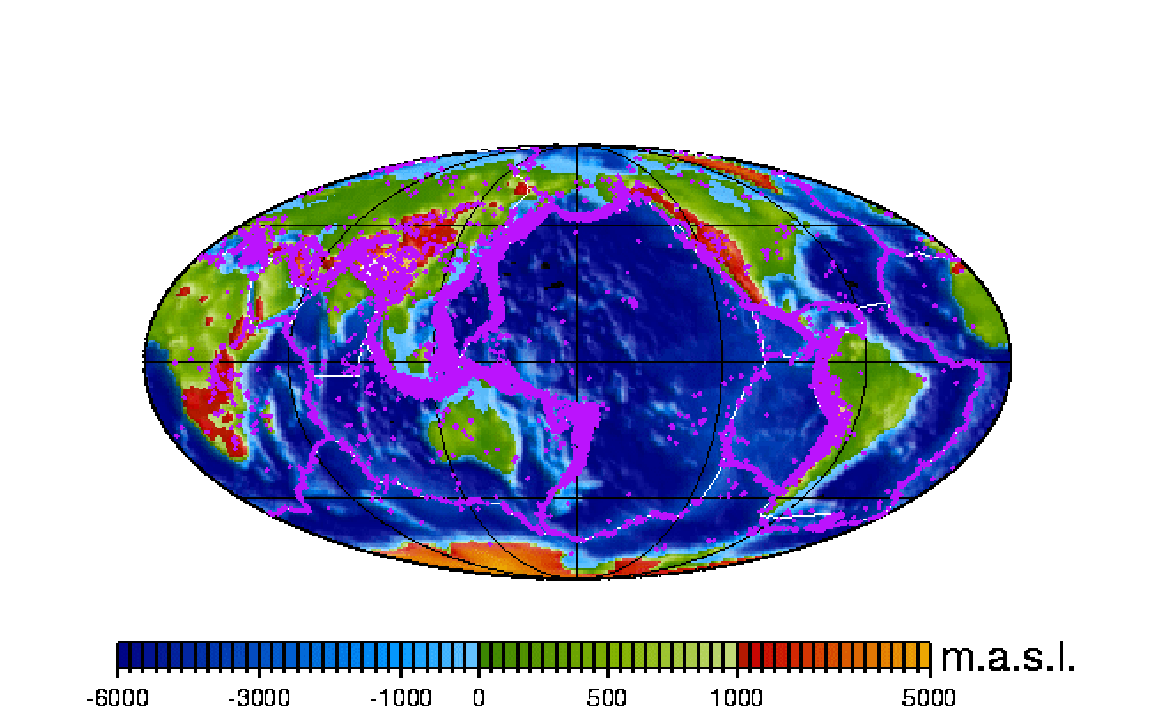
\includegraphics[height=8cm]{./examples/example1}}
\caption{ETOPO5, NUVEL1 plate boundaries and PDE hypocenter
  distribution as of {\tt example1.ps}, 
  resolution reduced. Data from \cite{demets90,etopo5,usgsneic}. 
  \label{fig1}}
\end{figure}

Figure~\ref{fig1} shows the map of \url{example1.ps} from the iGMT
distribution, the whole Earth in the Mollweide projection. ETOPO5 in
60 arc minute resolution is the ground raster layer. All hypocentres
of the USGS/NEIC dataset from 1973 -- 1997 with magnitude greater than
five and NUVEL1 plate boundaries are superimposed. Load {\tt
  example1.dat} to produce this plot. To reduce the size of this
documentation, the postscript file is not exactly that produced by
iGMT but a converted GIF with lower resolution.

\paragraph{Smith \& Sandwell/GTOPO30 topography}

Figure~\ref{fig2} of example number two shows a part of the Indian
ocean and the Indian subcontinent. It was produced using the Smith \&
Sandwell/GTOPO30 dataset in full resolution and has the pscoast
shoreline data in high resolution superimposed. The original map has
fascinating detail that might be lost in this reproduction.
\begin{figure}
\centerline{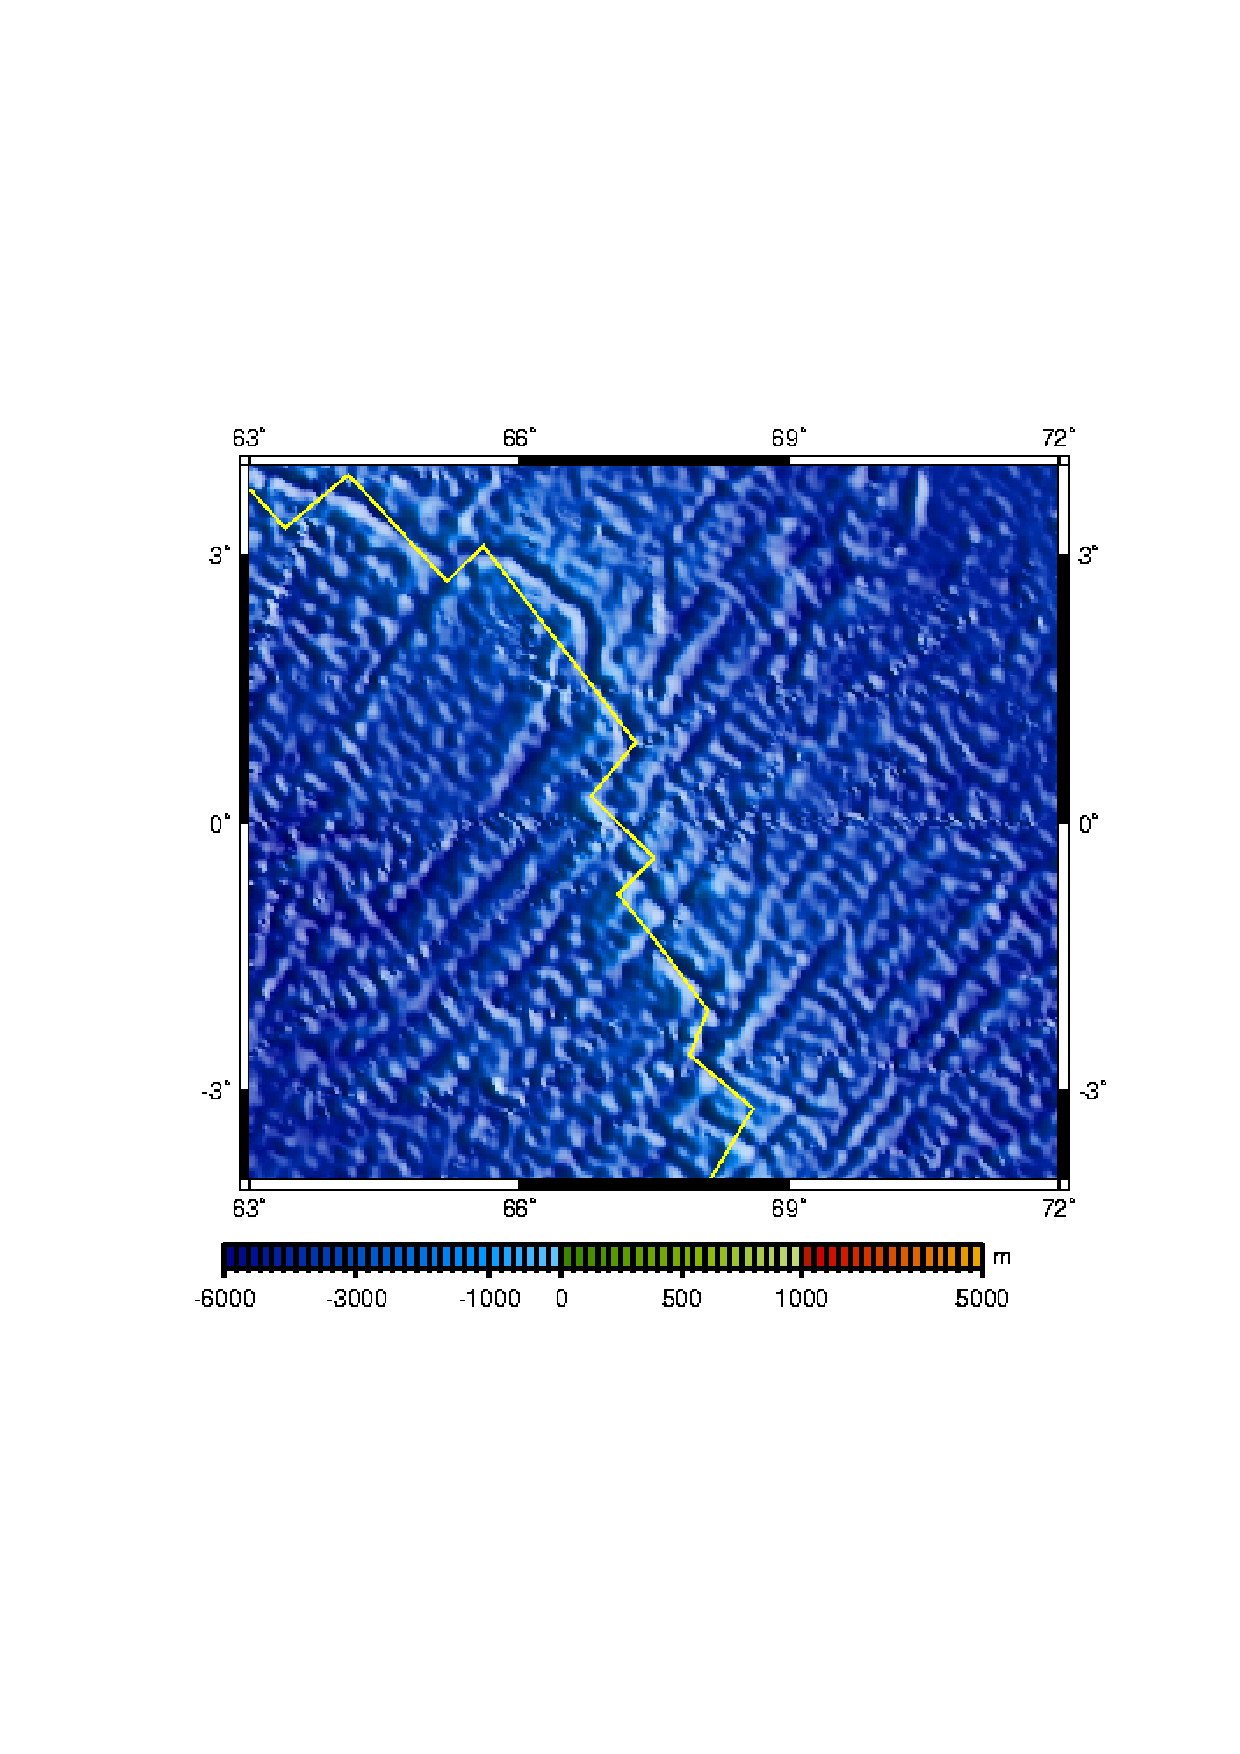
\includegraphics[height=8cm]{./examples/example2}}
\caption{A part of the Carlsberg ridge in the Indian Ocean as of 
  {\tt example2.ps},
  parameters can be loaded from {\tt example2.dat}. The original file
  has extremely high resolution and was quite big. The reduced
  image shown here was shrunk to 81dpi using {\tt xv}. Bathymetry data
  is from \cite{smith97}, plate boundary from \cite{demets90},
  scale is the same than in Fig.~\ref{fig1}. \label{fig2}}
\end{figure}


\paragraph{Sea-floor age of M{\"{u}}ller et al.}
\begin{figure}
\centerline{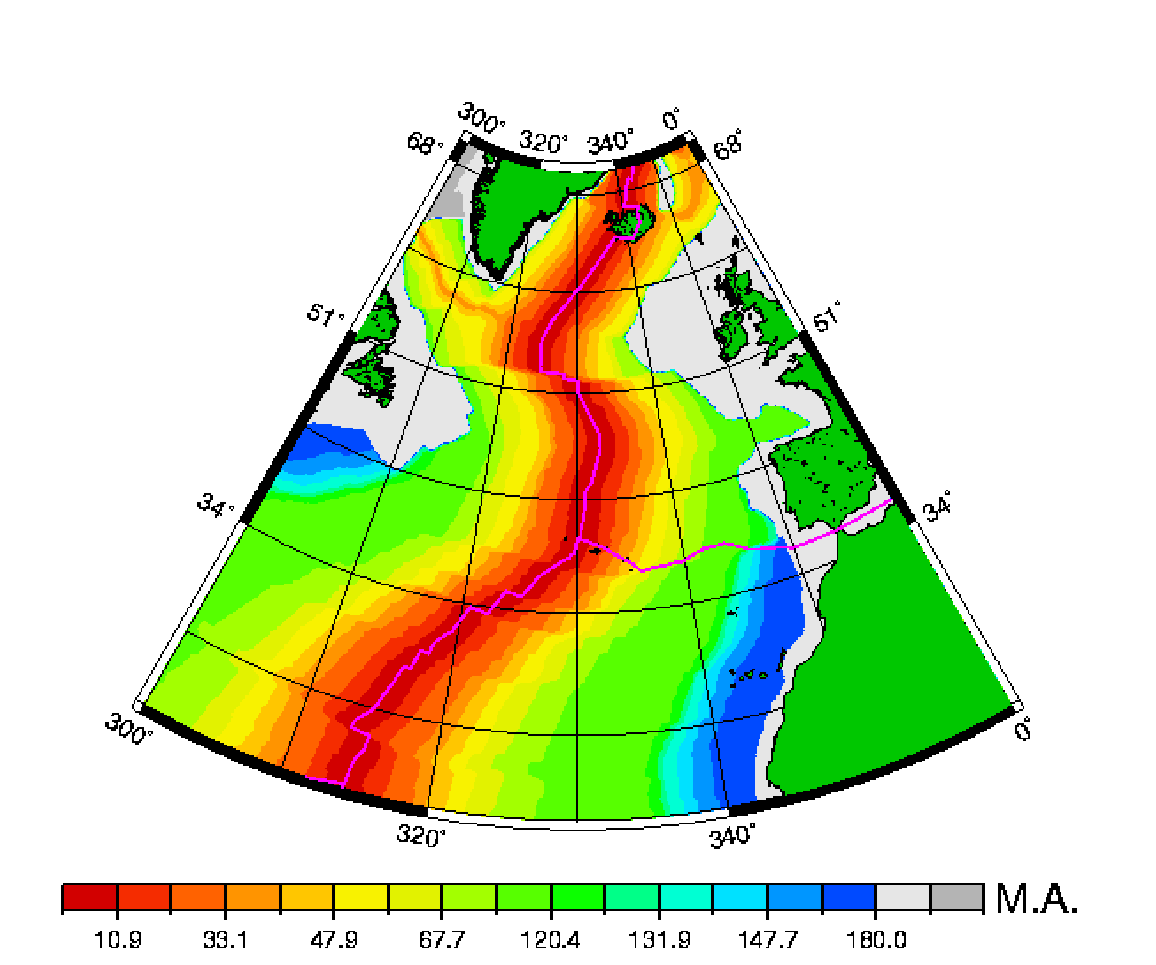
\includegraphics[height=8cm]{./examples/example3}}
\caption{Sea-floor age version 1.3 of \cite{mueller97} and plates from
  \cite{demets90}.\label{fig3}} 
\end{figure}
Example 3 as resp-resented by Fig.~\ref{fig3} and the files {\tt
  example3.ps} and \url{example3.dat} shows the North Atlantic region
sea-floor age data coverage together with plate boundaries
(Stereographic projection).



\paragraph{Gravity anomalies from \cite{sandwell97}}
\begin{figure}
\centerline{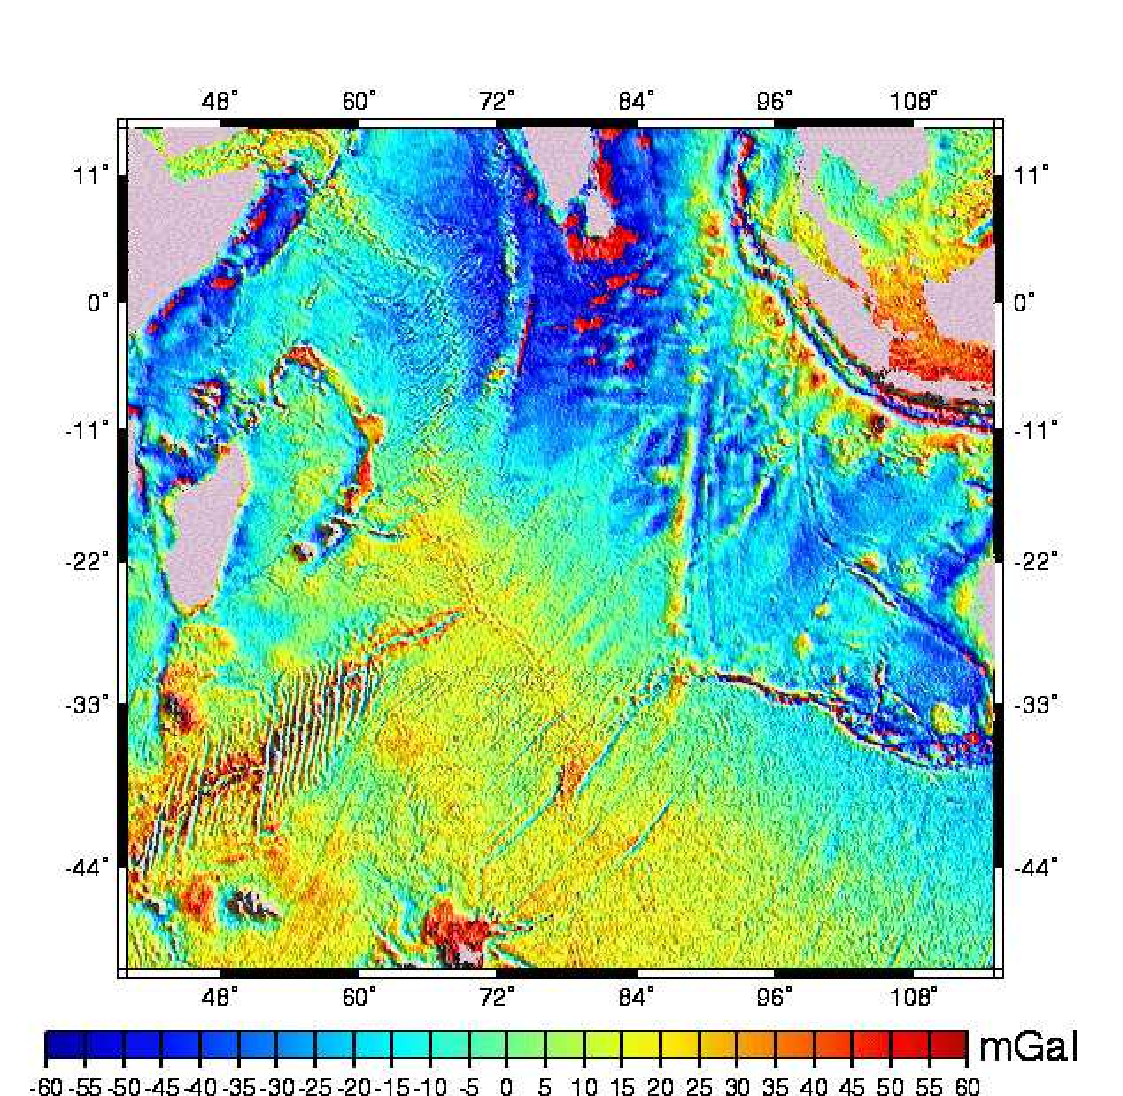
\includegraphics[height=8cm]{./examples/example4}}
\caption{Free-air gravity anomalies in a part of the Indian ocean from
  \cite{sandwell97}. Dominant features are the Carlsberg, 
  Southwest Indian and Southeast Indian ridges, the Bengal fan and the
  Ninety-east ridge. Resolution was restricted to 10 instead of 2 arc minutes.
  \label{fig4}}
\end{figure}
The last example (\url{example4.*}) of Fig.~\ref{fig4} shows gravity
anomalies in the Indian ocean. {\bf ATTENTION:} This example is quite
resource hungry and might lead to problems on smaller machines if
actually run with the original data set!

\clearpage
\section{Conclusion}

The iGMT software package was programmed in a modular way. Every
routine is commented, so it should be fairly easy to modify the code
and add extensions to the software. If you do so, that's fine, but
please do not call it iGMT when you distribute it and make reference
to the original software. Please keep in mind that while GMT offers a
large number of interesting and useful mapping options and iGMT tries
to make use of them, iGMT can't be as flexible as GMT. In addition, it
is pretty hard to test every single combination of
what-might-go-wrong-if. Hence, iGMT can be expected to fail to produce
useful maps under certain circumstances. Of course, the software is
provided as is, no guarantee whatsoever is given and no responsibility
for possible damage is taken.


Hopefully, iGMT demonstrates what can be done nowadays that great
geophysical data sets and mapping software is available. If iGMT helps
in making the research work of earth scientists easier, we are happy.

\bibliographystyle{apalike}

\addcontentsline{toc}{section}{\refname}
\bibliography{erdbeben}  


\clearpage
\hspace{0.5cm}{\bf {\Large {\flushleft \appendixname}}}

\appendix

\section{Technical details}

\subsection{Organization of the iGMT software}

After unpacking the \url{igmt_v1.2.tar} file the directory should look
something like this
\footnotesize

\begin{verbatim}
> ls -F
COPYING                          formatcpt.awk                    igmt_helper_create_ci_file*
COPYRIGHT                        igmt*                            igmt_helper_create_man_page*
INSTALL.TXT                      igmt.tcl                         igmt_helper_handle_gmtdefaults*
NOTES.TXT                        igmt_configure.tcl               igmt_helper_rmtmp_silent*
README.TXT                       igmt_datasets.tcl                igmt_init.tcl
colminmax.awk                    igmt_def.gif                     igmt_iomisc.tcl
colormaps/                       igmt_gmtdefaults_3.0             igmt_menus.tcl
configure_script*                igmt_gmtdefaults_3.1             igmt_parameters.tcl
example1.dat                     igmt_gmtdefaults_3.2             igmt_plotting.tcl
example2.dat                     igmt_gmtdefaults_3.3             img2grd*
example3.dat                     igmt_gmtdefaults_3.4             sortwsm.awk
example4.dat                     igmt_helper_checkfile*
\end{verbatim}
\normalsize
where the \url{colormaps} directory contains the color tables for GMT.
\footnotesize
\begin{verbatim}
> ls 
bathymetry.cpt     col.11.cpt         col.23.cpt         col.35.cpt         sediment.2.cpt
col.00.cpt         col.12.cpt         col.24.cpt         col.36.cpt         sediment.cpt
col.01.cpt         col.13.cpt         col.25.cpt         col.37.cpt         tomo.cpt
col.02.cpt         col.14.cpt         col.26.cpt         col.th.1.cpt       tomo2.cpt*
col.03.cpt         col.15.cpt         col.27.cpt         colgeoid.cpt       topo.bw.cpt
col.04.cpt         col.16.cpt         col.28.cpt         geoid.cpt          topo.cpt
col.05.cpt         col.17.cpt         col.29.cpt         geoid2.cpt         topo1.cpt
col.06.cpt         col.18.cpt         col.30.cpt         geoid3.cpt         topo2.cpt
col.07.cpt         col.19.cpt         col.31.cpt         geoid5.cpt         topo3.cpt
col.08.cpt         col.20.cpt         col.32.cpt         gravity.cpt        topo4.cpt
col.09.cpt         col.21.cpt         col.33.cpt         seafloor_age.cpt
col.10.cpt         col.22.cpt         col.34.cpt         seafloor_age2.cpt
\end{verbatim}
\normalsize

The files in this distribution can be classified as follows:

\paragraph{Copyright:} \url{COPYING} and \url{COPYRIGHT} deal with legal issues.
iGMT is distributed under the GNU public license but should be used in
accordance with the Student Pugwash Pledge, see the file {\tt
  COPYING}.
\paragraph{configure\_script:} This short script is supposed to take over the 
installation process as described in sec.~\ref{install}.

\paragraph{img2grd:} Script from the GMT distribution that is supposed to be a patch when 
\url{img2latlongrd} is not available, included starting from GMT
3.3.6.

\paragraph{The {\tt igmt} file:} A \url{bash} script that is used to
check if the environment variable \url{$igmt_root} and \url{wish} is
available at the places iGMT is looking. If all is fine, \url{wish}
is invoked with \url{igmt.tcl}. \url{igmt_def.gif} is the start-up
screen. 

\paragraph{Tcl files:} All files with the \url{tcl} extension contain
the tcl code that runs iGMT. \url{igmt.tcl} is the main file, it
contains \url{source} commands and builds up some frames. {\tt
  igmt\_configure.tcl} has all global variables and the default
settings for plotting whereas \url{igmt_init.tcl} handles the startup
sequence. The file \url{igmt_menu.tcl} holds the definition for the
main menu line and the procedures found in \url{igmt_datasets.tcl},
\url{igmt_parameters.tcl} and \url{igmt_plotting.tcl} correspond
roughly to all possible actions in the individual pull-down
menus. Finally, \url{igmt_iomisc.tcl} contains most of the input/output 
routines and some additional tcl procedures. 

All of these files should be fairly well commented so that we won't go
into any detail here. 

\paragraph{{\tt igmt\_helper\_} files} These contain small \url{bash}
scripts that are called by iGMT' tcl routines and handle more
operating system based processes. Most of them could be integrated
into the main tcl code but it seemed more transparent for possible
porting to other operating systems to keep them external. 



\paragraph{{\tt example.dat} and {\tt .ps}:} The \url{dat} files
contain the parameter dump that was created with iGMT after the
examples presented in section~\ref{examples} were produced. The
postscript files are packed with \url{gzip} and correspond to the
shrinked figures in this manual and are not identical to the real
postscript files produced (they were too big to be included in the
distribution).
\paragraph{Documentation and data}
The file \url{manual.ps} is the manual you are reading as a postscript
file.  \url{nuvel.yx} is the modified plate boundary polygon file
after \cite{demets90}, \url{01_02-98.cmt} contains the Harvard CMT
double couple fault plane solution for the first 60 days of 1998 as an
example, \url{vocanoes.dat} the volcano locations after
\cite{simkin94}, \url{allslabs_rum.gmt} the slab seismicity contours
of \cite{gudmundsson98} and \url{hotspots.dat} the hotspot list of
\cite{steinberger00b}.

\paragraph{Colormaps:} The \url{colormaps} directory contains the colormaps that are
used by iGMT to map the default datasets. \url{col.00.cpt} through
\url{col.35.cpt} are generic colormaps which span the data range from
$-1\ldots1$. If you want to convert these colormaps to suit your data,
use an awk script like \url{colminmax.awk} which comes with the iGMT
distribution.  \small
\begin{verbatim}
# script to convert the data range of colorscale files for GMT
# by rescaling
BEGIN{
  if(min==0)min=-1.;
  if(max==0)max=1.;
  mean=(max+min)/2.;
  range=(max-min)/2.;
  printevery=50;
}
{
  if(NR<256){
    if(printevery - NR > 0)
      print($1*range+mean,$2,$3,$4,$5*range+mean,$6,$7,$8,$9);
    else {
      print($1*range+mean,$2,$3,$4,$5*range+mean,$6,$7,$8,$9,"L");
      printevery=NR+printevery;
    }
  }
  else
    print($0);

}
\end{verbatim}
\normalsize
If your data sets contains values between $-2$ and 3, say, and you would like to use the
rainbow colored colorscale \url{col.13.cpt}, use\\\
\begin{center}
\url{awk -f $igmt_root/colminmax.awk min=-2 max=3 \ldots \\ $igmt_root/colormaps/col.13.cpt > new_colormap.cpt}. \\
\end{center}
Here, ``\ldots'' means that the above should be in one line.

Also, you might want to use the \url{grd2cpt} function of GMT that
can be accessed over \url{create colormap} menu item.


\section{Modifying iGMT}

iGMT may be freely modified and distributed as long as modified
versions are not called iGMT. There are plenty of easy possible future
enhancements one could think of, for instance interactive design of
colormaps, support of more complicated user data sets and multiple
layers of raster data. When this extensions become available, they
will be included in future versions. Some common modification (as
opposed to extension or enhancement) tasks are described below:

\paragraph{Using other path names for the data sets.} 

All pathnames to data locations are assigned in \url{igmt_configure.tcl}. 
All raster data sets have two variables assigned to them: {\tt
  raster\_data(i)} and \url{raster_colormap(i)}, they refer to the
location of the raster data set number \url{i} and the location of the 
default colormap, respectively. Simply add a line like
\url{set raster_data(3) "/home/user/gtopo30/topo_6.2.img"}
to your \url{igmt_siteconfig.tcl} file, if your GTOPO30 dataset
(number 3 internally) is in \url{/home/user/gtopo30/}. The equivalent
variables for polygon data are called \url{poly_data(i)}, and it is
simplest to search for the appropriated variable names in {\tt
  igmt\_configure.tcl}. 


\paragraph{Including new data sets.}

You will have to do these things: ({\bf to be expanded})

\begin{enumerate}

\item Add the data location and its parameters to the 
  \url{igmt_configure.tcl} file. 
  
  This should be easier now with version 1.2 since we have replaced
  most global variables for raster and polygon data issues with
  arrays, such that you can simply add one more entry at the back.
  Right now, raster data sets are reserved from 1 to 11, with the
  limit being set to (variable: \url{nr_of_raster_data}) 20 raster
  data sets in total. Polygon data sets are restricted to 25, and
  right now all sets up to 20 are filled.  Read through {\tt
    igmt\_configure.tcl} to see how the default data sets are
  implemented here.

  Parameters for raster data are: location of data file, default
  colormap, geographical limits (East, West, South, and North
  boundaries), integer boundaries only (on/off),  the maximum
  resolution (in arc minutes), and resampling at other than default
  grid spacing (on/off). For polygon data: location of data, symbol size, symbol
  color, \ldots

\item Add the data selection choice to the \url{Datasets} menus. This
  is done in \url{igmt_menues.tcl} and \url{igmt_datasets.tcl}.

\item Add the data plotting routine to \url{igmt_plotting.tcl},
  taking the old datasets as an example. Make use of the predefined
  standard procedures for raster data.

\end{enumerate}





\end{document}
